%!TEX encoding = UTF-8 Unicode
%!TEX root = ../lect-w11.tex

%%%


\Subsection{Generiska strukturer}

\begin{Slide}{Repetition: Typparametrar och generiska strukturer}
\begin{itemize}\SlideFontSmall
\item Med hjälp av \Emph{typparametrar} \Eng{type parameters} kan du skapa \Emph{generiska strukturer} \Eng{generic structures}.
\item Typparametrar skrivs inom hakparenteser, exempelvis: \code{ [T, U] }
\item Generiska strukturer fungerar för \emph{olika} typer, \Alert{okända} vid \Emph{deklaration}. 
\begin{Code}
case class Pair[A, B](a: A, b: B):  // A och B är obundna (fria) inom []
  def swap: Pair[B, A] = Pair(b, a) // A och B bundna då swap saknar []
\end{Code}
\pause
\item Kompilatorn säkerställer \Alert{korrekt} \Emph{användning} redan vid \emph{kompilering}.
\item På användningsplatsen i koden (vid anrop eller instansiering) \Emph{binds} typparametrar till ''verkliga'' typer enligt typsystemets regler. 
\begin{REPL}
scala> val p = Pair("hej", 42)
val p: Pair[String, Int] = Pair(hej,42)

scala> p.swap
val res0: Pair[Int, String] = Pair(42,hej)
\end{REPL}
\pause
\item Skriver du inte ut typerna försöker kompilatorn \Emph{härleda} \Eng{infer} dem.
\item Klassen \code{Pair} kallas även \Emph{typkonstruktor} \Eng{type constructor} då den ''verkliga'' typen skapas först vid användning \code{Pair[String, Int]}.
\end{itemize}
\end{Slide}


\Subsection{Att sätta gränser för typer}

\begin{Slide}{Olika sätt att begränsa typer}
Det finns i Scala flera olika sätt att att begränsa vilka typer du vill tillåta. En översikt av några möjligheter:
\begin{itemize}
  \item Ge \Emph{övre} gräns för typparametrar \Eng{lower bound}
  \item Ge \Emph{undre} gräns för typparametrar \Eng{upper bound}
  \item Ge en \Emph{kontextgräns} för typparametrar i relation till implicit givna typer \Eng{context bound}
  \item Begränsa möjlig inmixning vid deklaration av en trait med en explicit \Emph{egentyp} \Eng{self type} 
\end{itemize}
\end{Slide}

\begin{Slide}{Övre och undre typgränser}\SlideFontSmall
Med typoperatorerna \code{<:} och \code{>:} går det att begränsa vilka typer som kan bindas till en typparameter i en generiska struktur. 

\vspace{0.5em}Antag att \code{T} är en obunden typparameter medan \code{U} och \code{L} är bundna. 
\begin{itemize}
  \item med \code{T <: U} blir \code{U} en övre gräns \Eng{upper bound} för \code{T}\\(en ''högsta'' möjliga typ i  typhierarkin) 
  \item med \code{T >: L} blir \code{L} en undre gräns \Eng{lower bound} för \code{T}\\(en ''lägsta'' möjliga i  typhierarkin) 
  \item Minnesregel för typgränser: kolon på slutet.
  \item Alla typer \code{T} är implicit \code{T >: Nothing <: Any}
\end{itemize} 
\pause

\vspace{0.5em}Exempel: 
\begin{Code}
  trait Grönsak { def vikt: Int }

  def f[T <: Grönsak](x: T): Int = x.vikt
\end{Code}

Kompilatorn använder den övre typgränsen för att konstatera att metoden \code{vikt} är tillgänglig via den generiska parametern \code{x}.

\end{Slide}

\begin{Slide}{Exempel på övre och undre typgränser}

\begin{Code}
class Djur
class Katt extends Djur 
class Hund extends Djur
class Robothund extends Hund

def testUpperBound[T <: Hund](x: T) = println(x)
def testLowerBound[T >: Hund](x: T) = println(x)
\end{Code}

\begin{REPL}
scala> testUpperBound[Katt](Katt())
-- Error:
1 |testUpperBound[Katt](Katt())
  |          ^
  |          Type argument Katt does not conform to upper bound Hund

scala> testLowerBound[Robothund](Robothund())
-- Error:
1 |testLowerBound[Robothund](Robothund())
  |          ^
  |          Type argument Robothund does not conform to lower bound Hund
\end{REPL}

\end{Slide}


\Subsection{Flexibla generiska typer: varians}

\ifkompendium\else
\begin{SlideSimple}{Vad är varians?}
\hspace*{-2cm}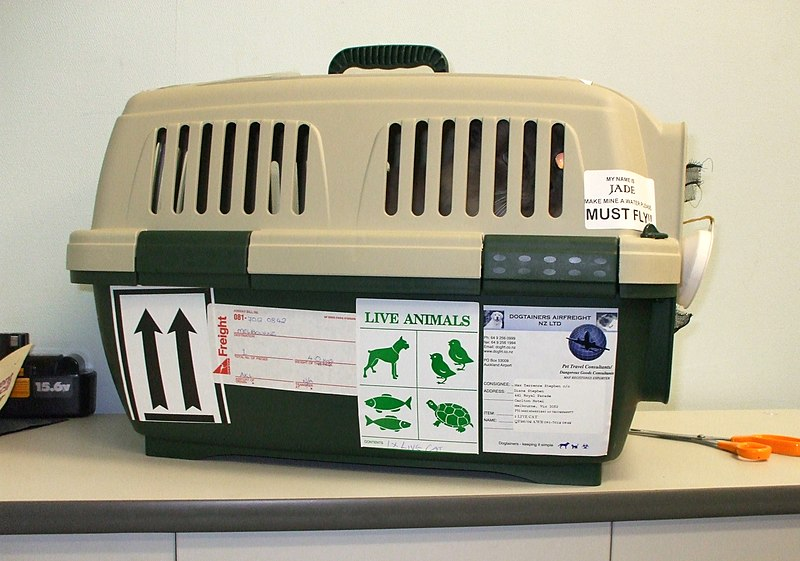
\includegraphics[width=1.4\textwidth]{../img/pet-carrier.jpg}  
\end{SlideSimple}
\fi 

\begin{Slide}{Vad är varians?}
\begin{center}
\textbf{Är en kattbur också en djurbur??}

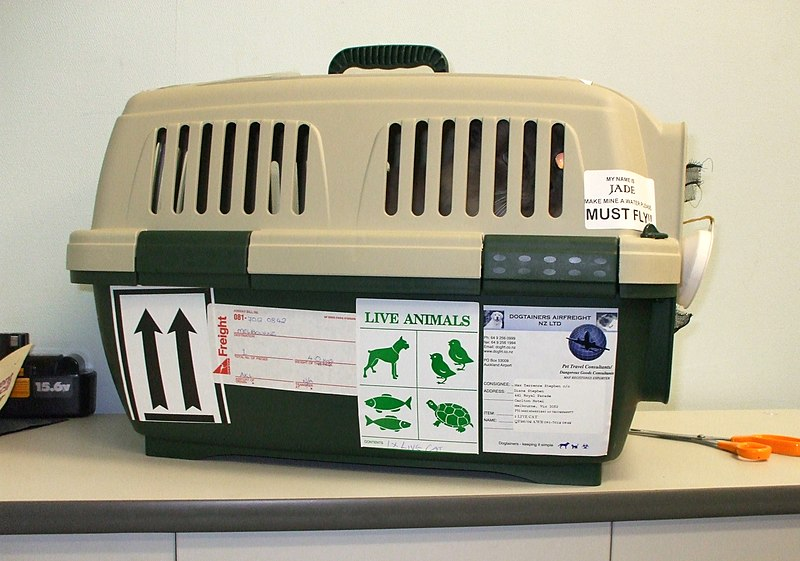
\includegraphics[width=0.75\textwidth]{../img/pet-carrier.jpg}  

Om vi tillåter \Emph{varians} så blir generiska strukturer mer \Alert{flexibla}.
\end{center}
\end{Slide}

\begin{Slide}{Varför behövs varians?}\SlideFontSmall
\begin{Code}
trait Djur
case class Katt() extends Djur
case class Hund() extends Djur

case class Bur[A](a: A)
\end{Code}
\pause
Nedan fungerar inte! Buren ovan är \Emph{invariant} (oflexibel i sin typparameter).
\begin{REPL}
scala> val djurbur: Bur[Djur] = Bur[Katt](Katt())
-- Error:
1 |val djurbur: Bur[Djur] = Bur[Katt](Katt())
  |                   ^^^^^^^^^^^^^^^^^
  |                   Found:    Bur[Katt]
  |                   Required: Bur[Djur]
\end{REPL}
\pause
Varför fungerar detta??
\begin{REPL}
scala> val djur: Vector[Djur] = Vector[Katt](Katt())
val djur: Vector[Djur] = Vector(Katt())
\end{REPL}
\pause \code{Vector} är deklarerad som \Emph{kovariant} och därmed mer flexibel!
\end{Slide}


\begin{Slide}{Kovarians \Eng{covariance}}
\begin{itemize}\SlideFontSmall
\item För en \Emph{kovariant} typkonstruktor \code{F} gäller att: 
\item[] \textbf{om} \code{ T <: U } \textbf{så} \code{ F[T] <: F[U] }~(subtypsflexibel ''på samma håll'')
\item I Scala kan du få en kovariant typkonstruktor med \code{+} före typparametern:
\begin{Code}
trait Djur
case class Katt() extends Djur
case class Hund() extends Djur

case class Bur[+A](a: A)  // kovariant tack vare + före A
\end{Code}
\pause
\item Nu funkar det \code{:)}
\begin{REPL}
scala> val djurbur: Bur[Djur] = Bur[Katt](Katt())
val djurbur: Bur[Djur] = Bur(Katt())
\end{REPL}
\item En kattbur är nu en \Alert{subtyp} till djurbur!
\pause
\item \Emph{Oföränderliga} samlingar görs ofta kovarianta, t.ex Vector, Option.
\item Enumerationer blir mer flexibla om du gör dem kovarianta:
\item[] \code|enum Toalett[+T] { case Upptagen(x: T); case Ledig }|
\end{itemize}

\end{Slide}


\ifkompendium\else
\begin{SlideSimple}{Kontravarians}
\hspace*{-1cm}
\includegraphics[width=1.2\textwidth]{../img/cat-vet.jpg}  
\end{SlideSimple}
\fi 

\begin{Slide}{Kontravarians}
\begin{center}
Är en kattveterinär också en djurveterinär?


\includegraphics[width=0.70\textwidth]{../img/cat-vet.jpg}  

Ibland vill vi ha variansen på andra hållet: En veterinär som bara kan behandla katter ska inte få behandla vilket djur som helst.
\end{center}
\end{Slide}

\begin{Slide}{Kontravarians \Eng{contravariance}}
\begin{itemize}\SlideFontSmall
\item För en \Emph{kontravariant} typkonstruktor \code{F} gäller att: 
\item[] \textbf{om} \code{ T <: U } \textbf{så} \code{ F[U] <: F[T] }~(subtypsflexibel ''på fel håll'')
\item Du skapar en kontravariant typkonstruktor med \code{-} före typparametern:
\begin{Code}
trait Djur 
case class Katt() extends Djur
case class Hund() extends Djur

class Veterinär[-A]:    // kontravariant med -
  def behandla(x: A) = println(s"$this har behandlat $x")  
\end{Code}
\pause
\item Nu funkar det ''baklänges'' (men inte på andra hållet):
\begin{REPLsmall}
scala> val kattveterinär: Veterinär[Katt] = Veterinär[Djur]()
val kattveterinär: Veterinär[Katt] = Veterinär@77b6d94c

scala> val kattveterinär: Veterinär[Djur] = Veterinär[Katt]()
-- Error:
1 |val kattveterinär: Veterinär[Djur] = Veterinär[Katt]()
  |                                     ^^^^^^^^^^^^^^^^^
  |                                     Found:    Veterinär[Katt]
  |                                     Required: Veterinär[Djur]
\end{REPLsmall}
\end{itemize}

\end{Slide}

\begin{Slide}{Variansproblem -- tack kompilatorn!}
\begin{itemize}\SlideFontSmall
\item En typkonstruktor kan \Alert{inte} vara kovariant om typparametern används som parametertyp för metoder (så kallad \emph{kontravariant position}):
\begin{Code}
trait Djur
case class Katt() extends Djur
case class Hund() extends Djur
\end{Code}
\begin{REPLsmall}
scala> case class Bur[+A](a: A): 
         def bytTill(x: A): Bur[A] = Bur(x)
-- Error:
2 |  def bytTill(x: A): Bur[A] = Bur(x)
  |          ^^^^
  |  covariant type A occurs in contravariant position in type A of parameter x
\end{REPLsmall}
\item Här måste typen tillåtas variera ''uppåt'' med hjälp av en \Emph{undre gräns}:
\begin{Code}
case class Bur[+A](a: A): 
  def bytTill[B >: A](x: B): Bur[B] = Bur(x)
\end{Code}
\begin{REPLsmall}
scala> Bur[Katt](Katt()).bytTill(Hund())
val res1: Bur[Djur] = Bur(Hund())
\end{REPLsmall}
\end{itemize}
\end{Slide}

\begin{Slide}{När använda vilken slags varians?}
\begin{itemize}\SlideFontTiny
\item Oföränderliga generiska klasser som har metoder som är \Emph{producenter} av nya oföränderliga generiska typer passar ofta bäst som \Emph{kovarianta}, t.ex. \code{Vector[+T]}, \code{Option[+T]} . 
\item En typkonstruktor av \code{T}, som har metoder som är \Alert{konsumenter} av \code{T}, kan vara flexibel i \code{T} om den är \Emph{kontravariant}, t.ex. \code{Veterinär[-T]}. Den kan också vara kovariant om konsumerande metoder vidgar inparametertypen till \code{B} där \code{B >: T}
\item En typkonstruktor med flera parametrar kan vara \Emph{både} kontravariant \Emph{och} kovariant, t.ex. \code{Function1[-A, +B]} \\-- detta är den egentliga typen bakom ''syntaktiska sockret'' \code{A => B}\\
(ett parametervärde\code{:A} \emph{konsumeras} och ett returtvärde\code{:B} \emph{produceras})
\item \Alert{Förändringsbara} strukturer måste vara \Emph{invarianta}, annars väntar \Alert{kaos}!\\
\pause Antag att det finns en \code{Bur} som kan ändras på plats via metoden \code{bytTill} \emph{och samtidigt} vore kovariant (varning för känsliga kodare): 
\begin{REPLsmall}
ejscala> val kattBur: Bur[Katt] = Bur(Katt())

ejscala> val djurBur: Bur[Djur] = kattBur  // en kovariant referens till samma Bur

ejscala> djurBur.bytTill(Hund())           // en djurbur kan innehålla hundar

ejscala> val katt: Katt = kattBur.släppUt  // KAOS! typosäkert hundkatt-monster :(
\end{REPLsmall}
\end{itemize}
\end{Slide}


\begin{Slide}{Typjoker \Eng{wildcard type}}\SlideFontSmall
\Emph{Invarianta} klasser har oflexibel typparameter, vilket begränsar användningen. %(mer om varians senare).
\begin{REPL}
scala> class Box[A](val value: A)

scala> val b: Box[Any] = Box[Int](42)
-- Error:
1 |val b: Box[Any] = Box[Int](42)
  |                  ^^^^^^^^^^^^
  |                  Found:    Box[Int]
  |                  Required: Box[Any]
\end{REPL}  
Tveksam räddning: En \Emph{typjoker} \Eng{wildcard type} skrivs med ett frågetecken och ger en helt okänd typ  som \Alert{ej kontrolleras av kompilatorn}.
\begin{REPL}
scala> var whatever: Box[?] = Box[Int](42)
var whatever: Box[?] = Box@70d7a49b
                                                                                    
scala> whatever = Box("hej")
whatever: Box[?] = Box@43120a77
\end{REPL}
Använd bara typpjoker om det \emph{verkligen} behövs.
\end{Slide}


\begin{Slide}{Mer om varians för den nyfikne}
\begin{itemize}\SlideFontSmall
  \item \href{https://docs.scala-lang.org/scala3/book/types-variance.html}{https://docs.scala-lang.org/scala3/book/types-variance.html}
  \item \href{https://en.wikipedia.org/wiki/Covariance_and_contravariance_(computer_science)}{https://en.wikipedia.org/wiki/Covariance\_and\_contravariance\_(computer\_science)}
  \item \href{https://www.artima.com/pins1ed/type-parameterization.html}{https://www.artima.com/pins1ed/type-parameterization.html}

\end{itemize}
\end{Slide}



\begin{Slide}{Typbegränsning med egentyp \Eng{self type}}\SlideFontSmall
\begin{itemize}\SlideFontTiny
  \item Det går att gå ett explicit, valfritt namn, t.ex. \code{self},  på ''mig själv'', alltså denna instans, genom att skriva~\code{ self => }~i kroppen på en trait eller klass. 
  \item En typbegränsning på den egna instansen kallas \Emph{egentyp} \Eng{self type}. 
  \item Användbart vid inmixning: du kan begränsa med vad denna trait får mixas in.
\begin{Code}
trait Grönsak { def vikt: Int }
trait KanSkalas:
  self: Grönsak =>
  def viktEfterSkalning = 0.99 * vikt 
\end{Code}
\begin{REPLsmall}
scala> val g = new Grönsak with KanSkalas { val vikt = 100 }
val g: Grönsak & KanSkalas = anon1@70a91d72
                                                                                    
scala> g.viktEfterSkalning
val res0: Double = 99.0
\end{REPLsmall}
\item Även om \code{KanSkalas} \Alert{inte} gör \code{extends} så är \Emph{ändå} \code{vikt} tillgänglig i dess kropp, eftersom vi kräver att den egna typen är en \code{Grönsak}.
\item Kan användas för att göra s.k. \Emph{beroendeinjektion} \Eng{dependency injection}.\\\url{https://en.wikipedia.org/wiki/Dependency_injection}
\end{itemize}

\end{Slide}



\Subsection{Kontextuella abstraktioner}


\begin{Slide}{Sammanhanget är avgörande när du kodar!}
\begin{itemize}\SlideFontSmall
  \item \Emph{Kontexten}, alltså sammanhanget, styr vilka namn som syns var.
  \pause
  \item \textbf{Objektorientering} (OO) skapar sammanhang med:
  \begin{itemize}\SlideFontTiny
    \item \Emph{Namnrymder}
    \item \Emph{Tillstånd}
    \item \Emph{Subtypspolymorfism}
  \end{itemize} 
  \pause
  \item \textbf{Funktionsprogrammering} (FP) skapar sammanhang med:
  \begin{itemize}\SlideFontTiny
    \item \Emph{Parametrar}
    \item \Emph{Funktionsvärden}
    \item \Emph{Parametrisk polymorfism}
  \end{itemize}
  \pause
  \item \textbf{Kombinationen} av OO och FP är \Emph{extra} kraftfull och flexibel!
  \pause
  \item Men det finns \Alert{svårigheter}:
  \begin{itemize}\SlideFontTiny
    \item OO: ibland svårt att resonera om ändrade tillstånd och dynamisk bindning
    \item FP: kan bli många parametrar som måste upprepas vid nästlade anrop
  \end{itemize} 
  \pause
  \item Till vår räddning, fler coola FP-grejer: 
  \begin{itemize}\SlideFontTiny
    \item \Emph{Kontextuella abstraktioner}: möjliggör (på annat ställe) \Emph{givna} värden som finns \emph{implicit} (alltså underförstått, utan att vi behöver explicit skriva ut dem).
    \item \Emph{Ad hoc polymorfism}: möjliggör olika implementationer beroende på typ, \emph{statiskt} härledda och utan att det behöver finnas en arvsrelation  
  \end{itemize} 
\end{itemize}
\end{Slide}

\begin{Slide}{Repetition: default-argument}\SlideFontSmall
\begin{itemize}\SlideFontSmall
\item Vi har tidigare sett att kompilatorn, med \Emph{default-argument}, kan \Alert{fylla i} värden, som vi inte måste skriva, vid funktionsanrop:
\begin{REPLnonum}
scala> def f(x: Int, y: Int = 42) = x + y
def f(x: Int, y: Int): Int

scala> f(1,2)        // explicit givet y-värde
val res0: Int = 3

scala> f(1)          // vi kan också skippa y-värdet  
val res1: Int = 43   // då används default-argumentet
\end{REPLnonum}
\end{itemize}
\end{Slide}


\begin{Slide}{Repetition: uppdelade parameterlistor}\SlideFontSmall
\begin{itemize}\SlideFontSmall
\item Vi har tidigare sett uppdelade parameterlistor, som möjliggör stegvis applicering (s.k. Curry-funktioner):
\begin{REPLsmall}
scala> def f(x: Int)(y: Int = 42) = x + y
def f(x: Int)(y: Int): Int

scala> val g = f(1)  // en ny funktion utan default-arg
val g: Int => Int = Lambda1352/0x08406d0840@dbc7e0a

scala> f(1)()   // y-värdet fylls i av kompilatorn
val res4: Int = 43
\end{REPLsmall}
\pause
\item  Kan vi ta detta ett steg till och \Alert{frikoppla} deklarationen av funktionen \Emph{från} det givna värdet, och ge detta på annan plats baserat på typen?
\pause 
\item I Scala 3 görs detta med nyckelorden \code{given} resp. \code{using}\\(i Scala 2 (över)användes nyckelordet \code{implicit})
\end{itemize}
\end{Slide}

\begin{Slide}{Givna värden som alternativ till default-argument}\SlideFontSmall
Exmpel på användning av \code{using} och \code{given}:
\begin{REPL}
scala> def f(x: Int)(using y: Int) = x + y
def f(x: Int)(using y: Int): Int

scala> f(1)(using 2)    //explicit värde används
val res0: Int = 3

scala> f(1)        // kompilatorn hittar inget givet Int-värde
-- Error:
1 |f(1)
  |    ^
  |  no implicit argument of type Int was found for parameter y of method f

scala> given Int = 42    // låt 42 vara givet 
lazy val given_Int: Int

scala> f(1)       // kompilatorn kan nu framkalla givet värde av typen Int
val res0: Int = 43
\end{REPL}
Det går också att ge det givna värdet ett namn vid behov, men ofta onödigt:\\
\code{given blabla: Int = 42}
\end{Slide}

\begin{Slide}{Kan vi inte använda default-argument som förändras?}
\begin{itemize}\SlideFontSmall
\item Vi skulle kunna använda ett default-värde som är ett namn på en variabel;
\begin{REPLsmall}
scala> var ctx = 42
var ctx: Int = 42

scala> def f(x: Int = ctx) = x + 1
def f(x: Int): Int

scala> f()
val res0: Int = 43

scala> ctx = 0

scala> f()                                                                      
val res1: Int = 1
\end{REPLsmall} 
\item Men här utgörs kontexten av referensen till ett föränderligt värde vid \Alert{körtid} som måste synas i aktuell namnrymd och \emph{inte} som för givna värden där det som fylls i baseras på \emph{typen} vid \Emph{kompileringstid} i en speciell \Emph{implicit namnrymd} \Eng{implicit scope}.
\end{itemize}
\end{Slide}
\begin{Slide}{Kontextuella abstraktioner med \texttt{given}, \texttt{using}}\SlideFontSmall
\Emph{Kontextuell abstraktion} \Eng{contextual abstraction} i Scala:
\begin{itemize}\SlideFontSmall
\item Nyckelordet \code{given} anger ett \Emph{givet värde} av en viss typ.
\item Värdet \Alert{framkallas} vid anrop med \Emph{kontextparameter} av given typ.
\end{itemize}
\begin{Code}
object MinKontext:
  given String = "tagen för givet"
  def framkalla(using s: String) = s  //kontextparametrar märks med using
\end{Code}
\pause\vspace{-0.9em}
\begin{REPLsmall}
scala> MinKontext.framkalla(using "explicit")
val res0: String = explicit

scala> given String = "ta denna"
lazy val given_String: String

scala> MinKontext.framkalla
val res1: String = ta denna

scala> import MinKontext.given String    // speciell import-syntax för givna värden

scala> MinKontext.framkalla
val res2: String = tagen för givet
\end{REPLsmall}
\end{Slide}

\begin{Slide}{Framkalla värde med \texttt{summon}}\SlideFontSmall
I standardbiblioteket för Scala 3 finns en generisk variant av metoden \code{framkalla} i föregående exempel, som är definierad så här:
\begin{Code}
def summon[T](using x: T) = x 
\end{Code}
Funktionen \code{summon} kan användas för att testa vilket värde kompilatorn framkallar i en viss kontext:
\begin{Code}
object MinKontext:
  given String = "tagen för givet"
\end{Code}
\vspace{-0.9em}
\begin{REPLsmall}
scala> summon[String]
-- Error:
1 |summon[String]
  |              ^
  | no implicit argument of type String was found for parameter x of 
  | method summon in object Predef. The following import might fix the problem:
  | import MinKontext.given_String

scala> import MinKontext.given    // importerar alla givna värden i MinKontext

scala> summon[String]
val res0: String = tagen för givet
\end{REPLsmall}
\end{Slide}

\begin{Slide}{Prioritetsordning vid framkallning av givna värden}\SlideFontSmall
\begin{itemize}\SlideFontSmall
\item Det kan finnas flera \Alert{olika} givna värden av \Emph{samma} typ.
\item Men då får det ju inte vara tvetydigt vilket implicit värde som ska väljas.
\item Därför väljer kompilatorn ett givet värde enligt denna prioritering:
\begin{enumerate}\SlideFontTiny
\item \Emph{Explicita} argument till kontextparametrar märkta med \code{using}
\item \code{given} och \code{import given ...} i aktuell namnrymd \Eng{current scope} 
\item \code{given}-värden i \Emph{kompanjonsobjekt} för den använda typen.
\item ... (fler knepiga regler som vi inte går in på här)
\end{enumerate}
\item Om flera givna värden kan framkallas för typer som ingår i en gemensam arvshierarki så väljer kompilatorn det givna värdet som är av den \emph{mest specifika} typen.
\end{itemize}
Framkallning av givna värden vid anrop med kontextparametrar har flera namn på engelska: \emph{to summon}, eller \emph{term inference}, eller \emph{implicit resolution}. 
\end{Slide}

\begin{Slide}{Ad hoc polymorfism, ''typklasser''}\SlideFontSmall
\begin{itemize}\SlideFontSmall
\item Ad hoc polymorfism innebär att en abstrakt typkonstruktor ges olika konkreta implementationer för olika typer och appliceras automatiskt. 
\item Uppfanns i språket ML och vidareutvecklades i språket Haskell.
\item I Haskell kallas Ad hoc polymorfism för ''typklasser''. \\(En förvirrande term; Haskell är inte objekt-orienterat...)
\item Ad hoc polymorfism / Typklasser görs i Scala genom att \Emph{kombinera} parametrisk polymorfism med kontextuella abstraktioner.
\end{itemize}
\begin{Code}
trait Parser[T]:
  def fromString(value: String): Option[T]

object Parser:
  given Parser[Int] with  // with behövs för givna instanser om abstrakt typ
    def fromString(value: String): Option[Int] = value.toIntOption   
\end{Code}
\begin{REPL}
scala> def parse[T](s: String)(using p: Parser[T]) = p.fromString(s)

scala> parse[Int]("12")
val res0: Option[Int] = Some(12)
\end{REPL}
\end{Slide}

\begin{Slide}{Parameternamnet kan skippas efter \texttt{using}}
\begin{itemize}
\item Eftersom namnet på det givna värdet ofta inte behövs\\ -- det är ju typen som är det viktiga för framkallningen, \\ så kan du skippa parameternamnet:%

\begin{Code}[basicstyle=\ttfamily\SlideFontSize{10}{14}\selectfont]
def parse[T](s: String)(using Parser[T]) = 
  summon[Parser[T]].fromString(s)
\end{Code}
\item Framkallningen kan vid behov istället%
\footnote{Ett vanligt parameternamn är annars \code{ev} som är en förkortning av \emph{evidence}, vilket anspelar på att kompilatorn -- om koden kompilerar utan fel -- har hittat ett giltigt \emph{bevis} för att det givna värdet verkligen existerar \textbf{vid anrop}.}
 göras med \code{summon}%

\end{itemize}
\end{Slide}


\begin{Slide}{Hur få ''typklassen'' \texttt{Parser} att funka för fler typer?}
\begin{REPL}
scala> parse[java.awt.Color]("Color(120,10,0)")
-- Error:
1 |parse[java.awt.Color]("Color(120,10,0)")
  |                                        ^
  | no implicit argument of type Parser[java.awt.Color] was found 
  | for parameter p of method parse
\end{REPL}
\begin{Code}
given Parser[java.awt.Color] with
  def fromString(value: String): Option[java.awt.Color] =
    val trimmed = value.trim.stripPrefix("Color(").stripSuffix(")")
    trimmed.split(",").map(_.toIntOption) match
      case Array(Some(r), Some(g), Some(b)) => Some(java.awt.Color(r, g, b))
      case _ => None
\end{Code}
\begin{REPL}
scala> parse[java.awt.Color]("Color(120,10,0)")
val res1: Option[java.awt.Color] = Some(java.awt.Color[r=120,g=10,b=0])
\end{REPL}
\end{Slide}


\begin{Slide}{Kontextgränser}\SlideFontSmall
Denna form av \code{using}-parametrar...
\begin{Code}
def parse[T](s: String)(using p: Parser[T]) = ???
\end{Code}
...där en typkonstruktor för typparametern ska framkallas är så pass vanlig att Scala erbjuder ett kortare och mer lättläst skrivsätt:
\begin{Code}
def parse[T: Parser](s: String) = ???
\end{Code}
Om \code{F[A]} är en typkonstruktor och du skriver \code{[T: F]} så blir \code{F} en så kallad \Emph{kontextgräns} \Eng{context boundary}. 
Kompilatorn expandera detta automatiskt till kontextparametern \code{(using F[T])}
\end{Slide}



\begin{Slide}{Ännu smidigare användning med extensionsmetod}\SlideFontSmall
Kombinera kontextgräns med extensionsmetod och få smidig punktnotation.
\begin{Code}
extension [T: Parser](s: String) 
  def parseOrElse(default: T): T = 
    summon[Parser[T]].fromString(s).getOrElse(default)
 
\end{Code}
\begin{REPL}
scala> "12".parseOrElse(42)
val res2: Int = 12

scala> "gurka".parseOrElse(42)
val res3: Int = 42

scala> "Color(100,100,0)".parseOrElse(java.awt.Color.black)
val res4: java.awt.Color = java.awt.Color[r=100,g=100,b=0]
\end{REPL}
Extensionsmetoder kan skrivas i efterhand på valfri plats och även göras tillgängliga med import.
\end{Slide}






\begin{Slide}{Sortera samlingar med given ordning}\SlideFontSmall
\begin{REPLsmall}
scala> case class Gurka(namn: String, vikt: Int)
                                                                                                                                            
scala> val xs = Vector(Gurka("a", 100), Gurka("b", 50), Gurka("c", 100))
val xs: Vector[Gurka] = Vector(Gurka(a,100), Gurka(b,50), Gurka(c,100))
                                                                                                                                            
scala> xs.sorted
-- Error:
1 |xs.sorted
  | ^
  | No implicit Ordering defined for B
  | where: B is a type variable with constraint >: Gurka

\end{REPLsmall}
\pause
Detta kan fixas genom att tillhandahålla en given ordning för \code{Gurka}:
\begin{Code}
given Ordering[Gurka] with
  def compare(x: Gurka, y: Gurka): Int =
    if (x == y) then 0 
    else if x.vikt < y.vikt then -1 
    else 1
\end{Code}
\begin{REPL}
scala> xs.sorted   // nu funkar det :)
val res0: Vector[Gurka] = Vector(Gurka(b,50), Gurka(a,100), Gurka(c,100))
\end{REPL}
\end{Slide}

\begin{Slide}{Sortera samlingar med ännu smidigare given ordning}\SlideFontSmall

\begin{Code}
given Ordering[Gurka] = Ordering.fromLessThan((g1, g2) => g1.vikt < g1.vikt)
\end{Code}


\begin{itemize}
  \item Det är vanligt att man vill ge ordningar.
  \item Därför finns en smidig hjälpmetod i kompanjonsobjektet för typklassen \code{Ordering} som heter \code{fromLessThan}
  \item Den tar som inparameter en funktion som tar två instanser och returnerar en boolean som är true om den första är ''mindre'' (alltså kommer före) enligt valfri definition. 
  \item Den returnerar en \code{Ordering} som kan erbjudas som ett givet värde.
\end{itemize}

\end{Slide}

\Subsection{Vad är ett bra api?}
\begin{Slide}{Vad är ett bra api?}
\begin{itemize}\SlideFontSmall
  \item Ett api \Eng{Application Programming Interface} är ett gränssnitt för applikationsprogrammering.
  \item Med ''gränssnitt'' menas att det (i koden) finns en gräns mellan vad som syns utåt och vad som finns innanför ''under huven''.
  \item Det finns många kvalitetsaspekter som är önskvärda för ett api:
\begin{itemize}\SlideFontSmall
  \item Enkelt att använda på utsidan även om insidan är komplex.
  \item Vadå ''enkelt att använda''?
  \begin{itemize}\SlideFontTiny
  \item Lätt att lära
  \item Lätt att komma ihåg
  \item Lätt att begripa
  \item Najs upplevelse (subjektivt)
  \end{itemize}  
  \item Löser ett (generellt) problem på ett bra sätt. Vadå ''bra''?
  \begin{itemize}\SlideFontTiny
    \item Snabbt (hög prestanda)
    \item Snålt (effektiv användning av resurser, t.ex. minne)
    \item ...
  \end{itemize}  
\end{itemize}
\item Intressant föredrag av Joshua Bloch (Google), om god api-design:
   \begin{itemize}\SlideFontTiny
\item
\url{https://research.google.com/pubs/archive/32713.pdf}
\item \url{https://youtu.be/aAb7hSCtvGw}
\end{itemize}
\end{itemize}
\end{Slide}

\begin{Slide}{Api-desgin med Scala}
\begin{itemize}\SlideFontSmall
\item Kombinera paradigm OO+FP för att välja bäst lämpade lösningen.
\item Avancerade abstraktionsmekanismer som kan vara utmanande för api-konstruktören men samtidigt bli enkelt för api-användaren
\item Gör det möjligt att skapa ett api som fungerar i flera körmiljöer:
   \begin{itemize}\SlideFontTiny
   \item På desktop och i back-end med JVM och Graal VM
   \item I front-end i webbläsaren med Scala JS
   \item Direkt till plattformsspecifik maskinkod med Scala Native
   \end{itemize}
\item Avancerade saker som vi inte gått in på i kursen men som kan hjälpa api-konstruktörer att göra lättanvänt api:
   \begin{itemize}\SlideFontTiny
   \item Metaprogrammering
   \item Typklassderivering
   \item Kontextfunktioner
   \item Opaka typer
   \item Explicita null-typer
   \item Lambda på typnivå och match-typer
   \item ...
\end{itemize}
\end{itemize}
\end{Slide}

\ifkompendium\else
\begin{Slide}{Köpa ett api för 55 miljarder?}
\hspace*{-0.7cm}
\includegraphics[width=1.1\textwidth]{../img/ericsson-buy-api.png}

{ \vspace{2em} Sydsvenskan 2021-11-23 }
\end{Slide}
\fi




